% !TEX root = ../../../main.tex
% 来源：中学数学实验教材·第三册（高中数学）
% 章节：二次函数 / 和二次函数有关的课题
% 原始文件：5.tex，行 1905-1932
% 类型：tikz
% ---
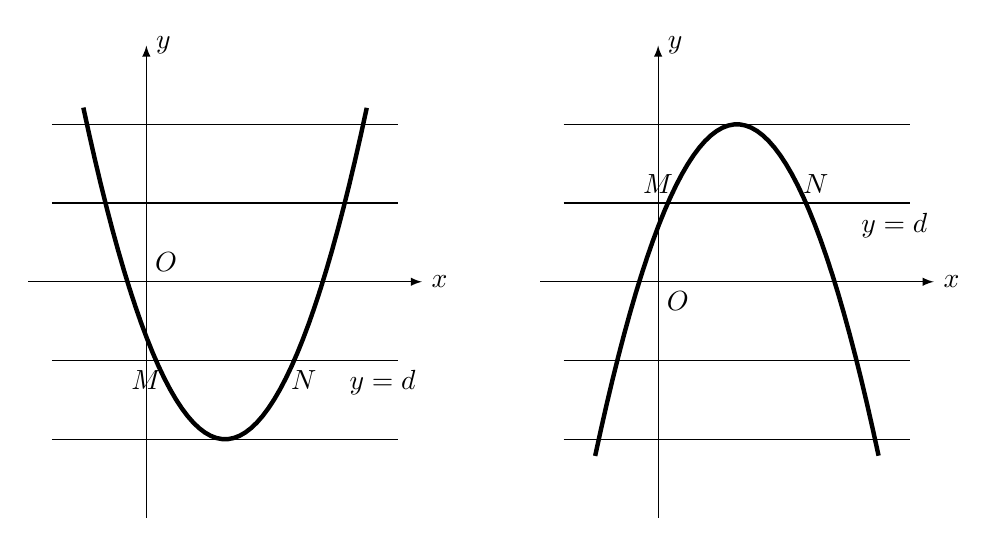
\begin{tikzpicture}[>=latex]
\begin{scope}
    \draw[->] (-1.5,0)--(3.5,0)node[right]{$x$};
    \draw[->] (0,-3)--(0,3)node[right]{$y$};
    \draw [domain=-.8:2.8, samples=50, ultra thick] plot(\x, {1.3*(\x-1)*(\x-1)-2});
    \foreach \x in {-2,-1,1,2}
    {
        \draw (-1.2,\x)--(3.2,\x);
    }
    \node at (3,-1)[below]{$y=d$};
    \node at (0,-1)[below]{$M$}; 
    \node at (2,-1)[below]{$N$};
    \node at (.25,.25){$O$};
\end{scope}

\begin{scope}[xshift=6.5cm]
    \draw[->] (-1.5,0)--(3.5,0)node[right]{$x$};
    \draw[->] (0,-3)--(0,3)node[right]{$y$};
    \draw [domain=-.8:2.8, samples=50, ultra thick] plot(\x, {-1.3*(\x-1)*(\x-1)+2});
    \foreach \x in {-2,-1,1,2}
    {
        \draw (-1.2,\x)--(3.2,\x);
    }
    \node at (3,1)[below]{$y=d$};
    \node at (0,1)[above]{$M$}; 
    \node at (2,1)[above]{$N$};\node at (.25,-.25){$O$};
\end{scope}
\end{tikzpicture}
